\documentclass{article}
\usepackage{graphicx}
\usepackage{multirow}
\usepackage{caption}
\usepackage{url}
\usepackage[utf8]{inputenc}
  \usepackage[
    backend=biber,
    style=ieee,
  ]{biblatex}
 
\addbibresource{references.bib}
\DeclareUnicodeCharacter{2212}{-}

\title{CS6000 - Second Assignment}
\author{Marc Moreno Lopez}
\date{September 10th 2018}

\begin{document}

\maketitle

\section{Introduction}

%Choose a “top” journal or conference in your field with >= 45 papers one or two 2016/2017/2018 issues.   (DO NOT search for papers with keywords.. but can search for journals/conf title).

%DONE

%Browse at least 45 papers in from that issue/issues, in order. No skipping or searching for keywords.

%DONE

%Time yourself on each, aim for no more than 2 min.  

%DONE

%Generate a bibtex entry for each paper, with a "note=" field that contains your timing (to the second) for your browse of that paper, and your decision to scan or trash it and 1 sentence why.  Do not time making that note"

%DONE

%Scan 8+ papers,  write 2-3 sentence summary, which is added to your "note" for that paper

%DONE

%Critically & Creatively read best  2 or 3.

%DONE

%Make a latex document with 3 sections.

%The first section in the journal  should   discuss your  process and your learning about the process (not the papers).

Browsing through many papers at once and deciding if it is worth your time or not can be a difficult task. During Summer 2016, I took an independent study with Dr. Kalita and I learned a lot about this. When I first browse a paper, I look at where the authors are from (where they work at), keywords (if they have any), the abstract, figures in the paper and results. First of all, the authors help me notice if it's a paper from a source that I already know. If it is, or I have already seen the author's name before, I'll probably scan that paper. Then, if the authors have included them, I'll look at the keywords. They are a good way to know if the paper is going to be related to an area that interests me. This is a good indicator of what I'm going to find in the abstract. Next, I read the abstract to get an idea of the work that they have done. If it is in an are that doesn't concern me, I'll automatically discard it. It also helps me to see if they have reported any results. Afterwards, I look at the figures to get a better idea of the method and ideas that have been used in the paper. Finally, I look at the results. This last stage is critical. If the results aren't properly reported, maybe the paper isn't worth reading. So it is a good indicator if a paper goes to the scanning phase or not. 


When I scan a paper, my methodology is a bit different. I focus more on the related work, method, results and conclusions. I like to get a good and clear idea of what the authors are doing and if their work is an improvement over the existing work. To do so, I start by looking at the related work section and look at what they state is different in their work from what has been previously done. After that, I skim through the method section, looking for their novel proposals and looking for the key parts of their algorithm. Then, I go to the conclusions section and see what they have stated. I look at the conclusions before looking at the results because then, when I look at the results section, I can see if their results confirm their conclusions or no. Once I have looked at the results section, I have a better idea if their work is significant or not. Finally, once I have a better idea of all the key points from the paper, I decide if that paper is worth a 3rd and 4th reading. To decide this I also take into account if the paper is related to my work or not and how much time and effort it will take me to read it and fully understand it.

%The second section is  your raw notes from critical/creative reads as a latex document, and include all the papers in the references. Not expecting/wanting full sentences, grammar, want your raw notes.  If you use handwritten notes, you can take pic and include them as figures.   

The first paper that I have decided to critically and creatively read is the one from M. Liu et al. \cite{10.1007/978-3-319-66179-7_1}. I have made handwritten notes, so I'll include them in figures.

\begin{figure}[h]
\centering
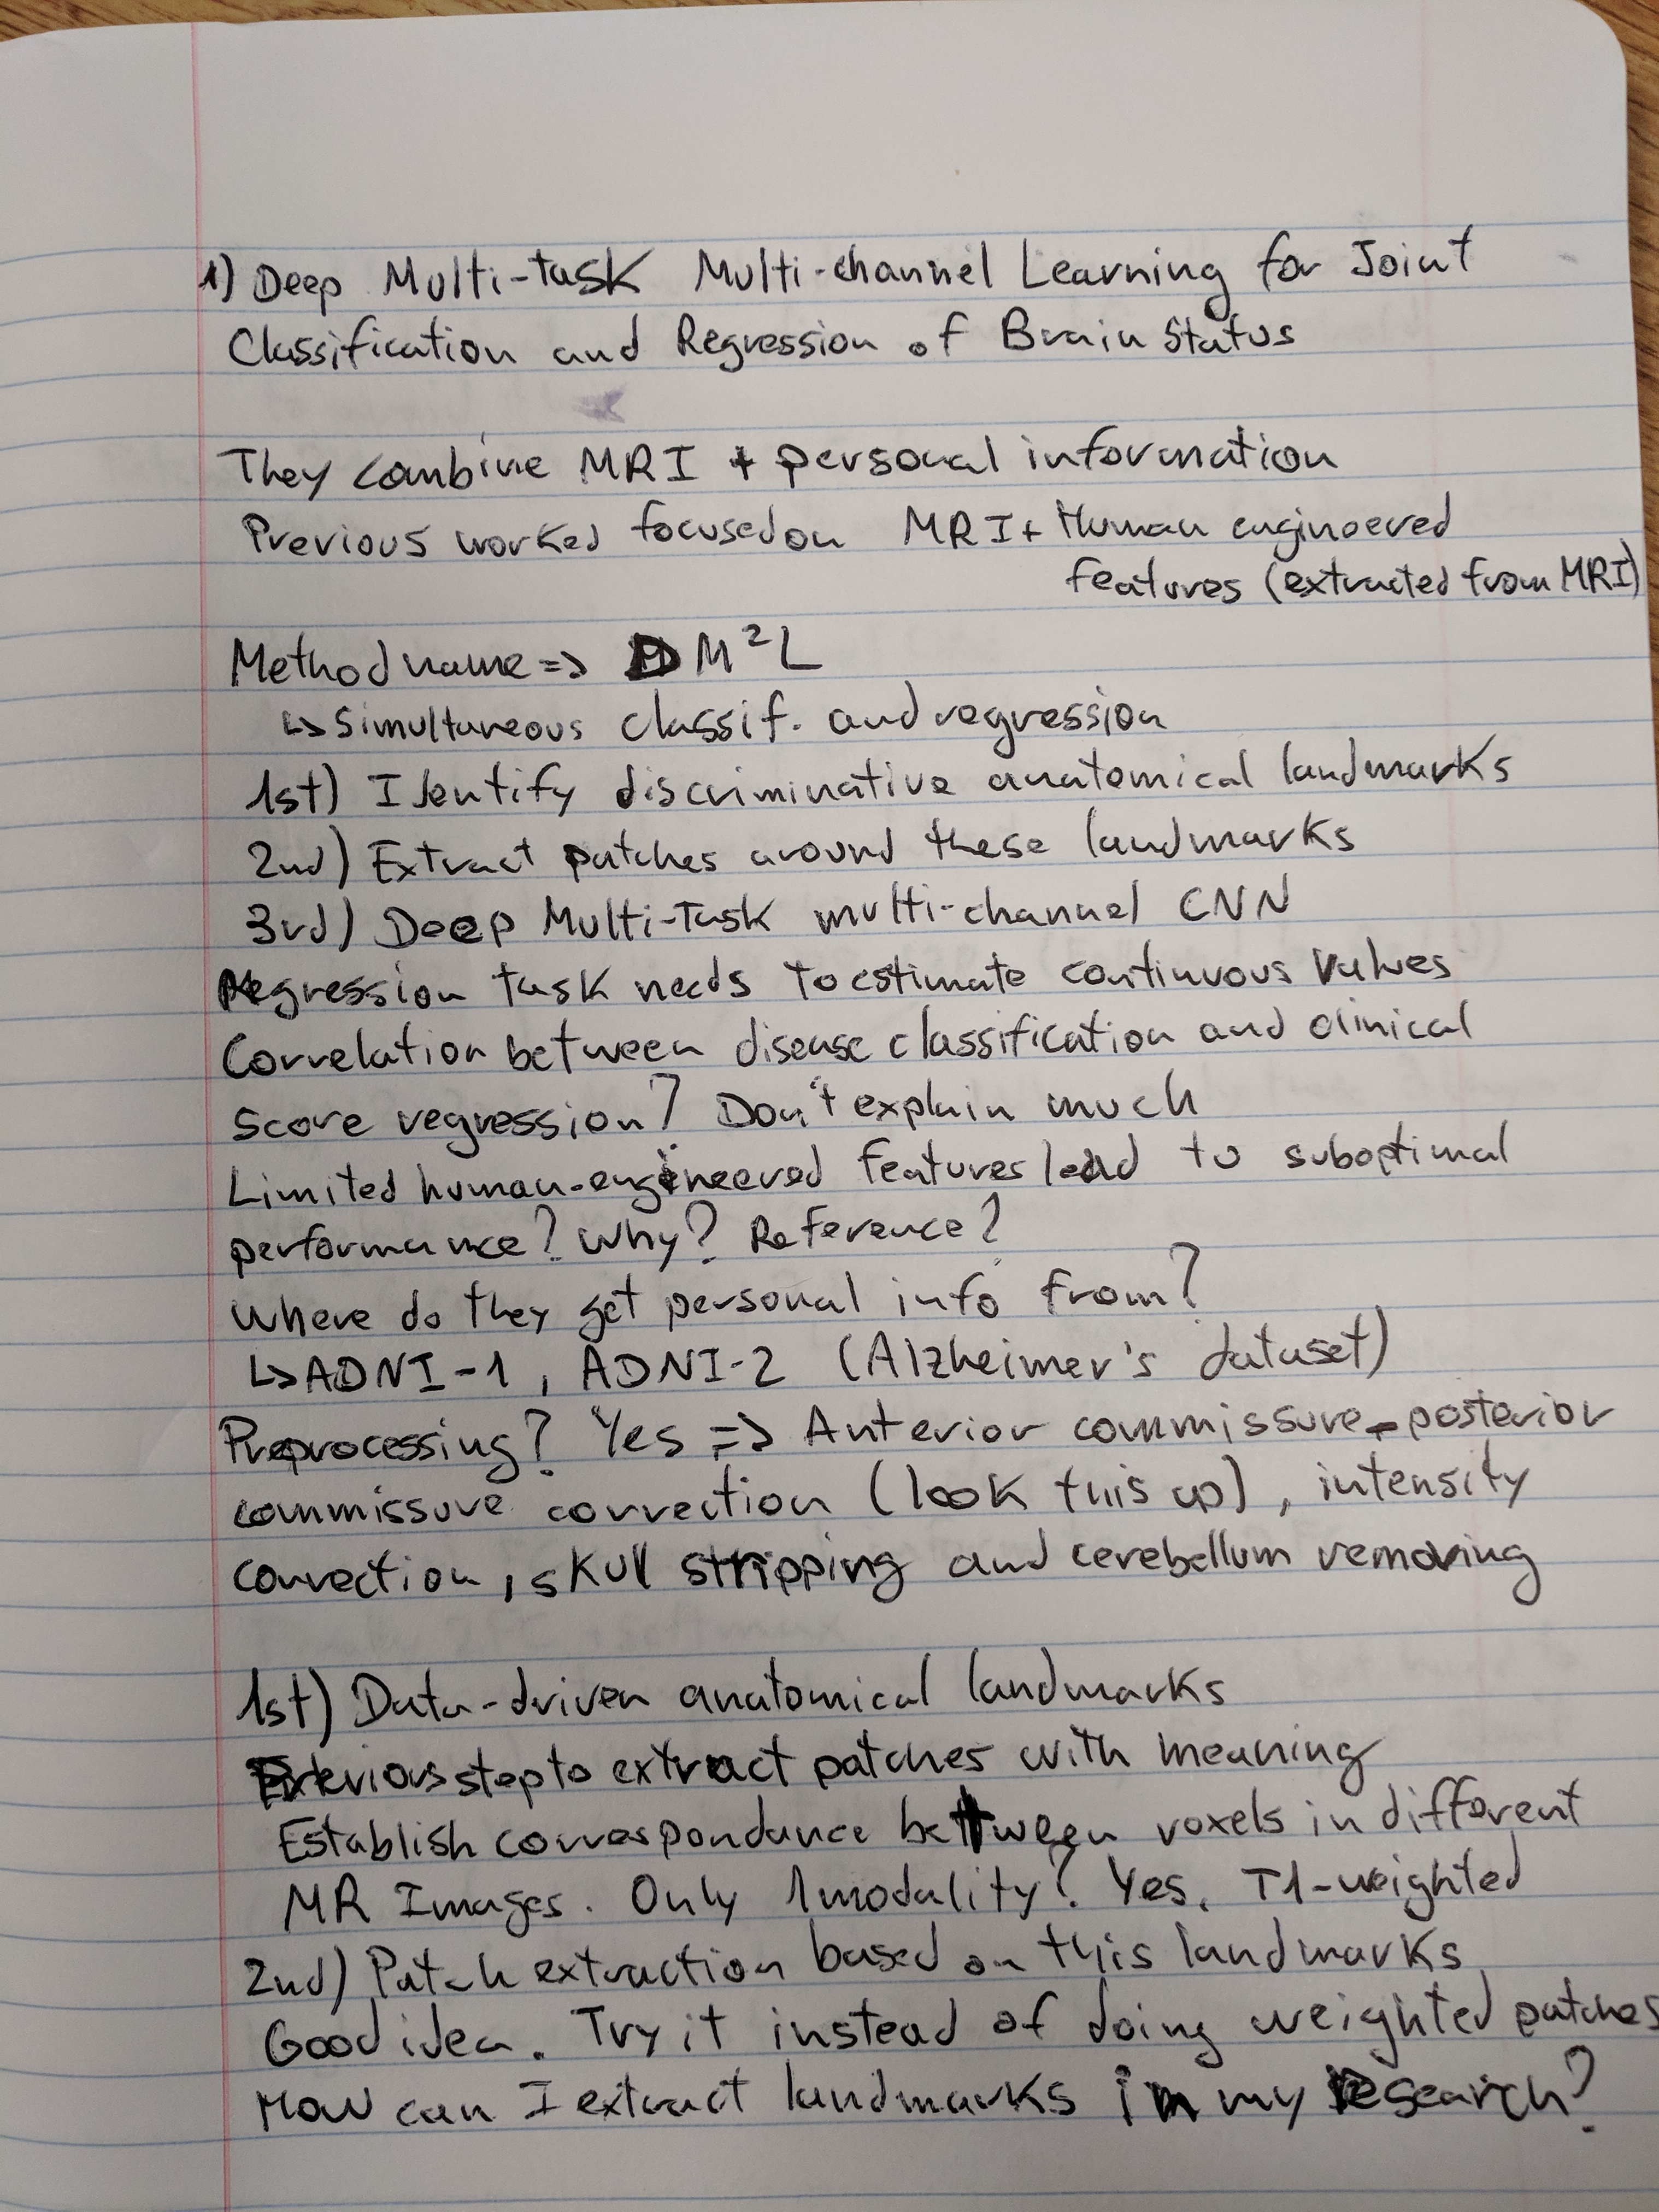
\includegraphics[width=10cm]{paper1_1.jpg}
\caption{Picture 1 for first paper}
\label{fig:paper1_1}
\end{figure}

\begin{figure}[h]
\centering
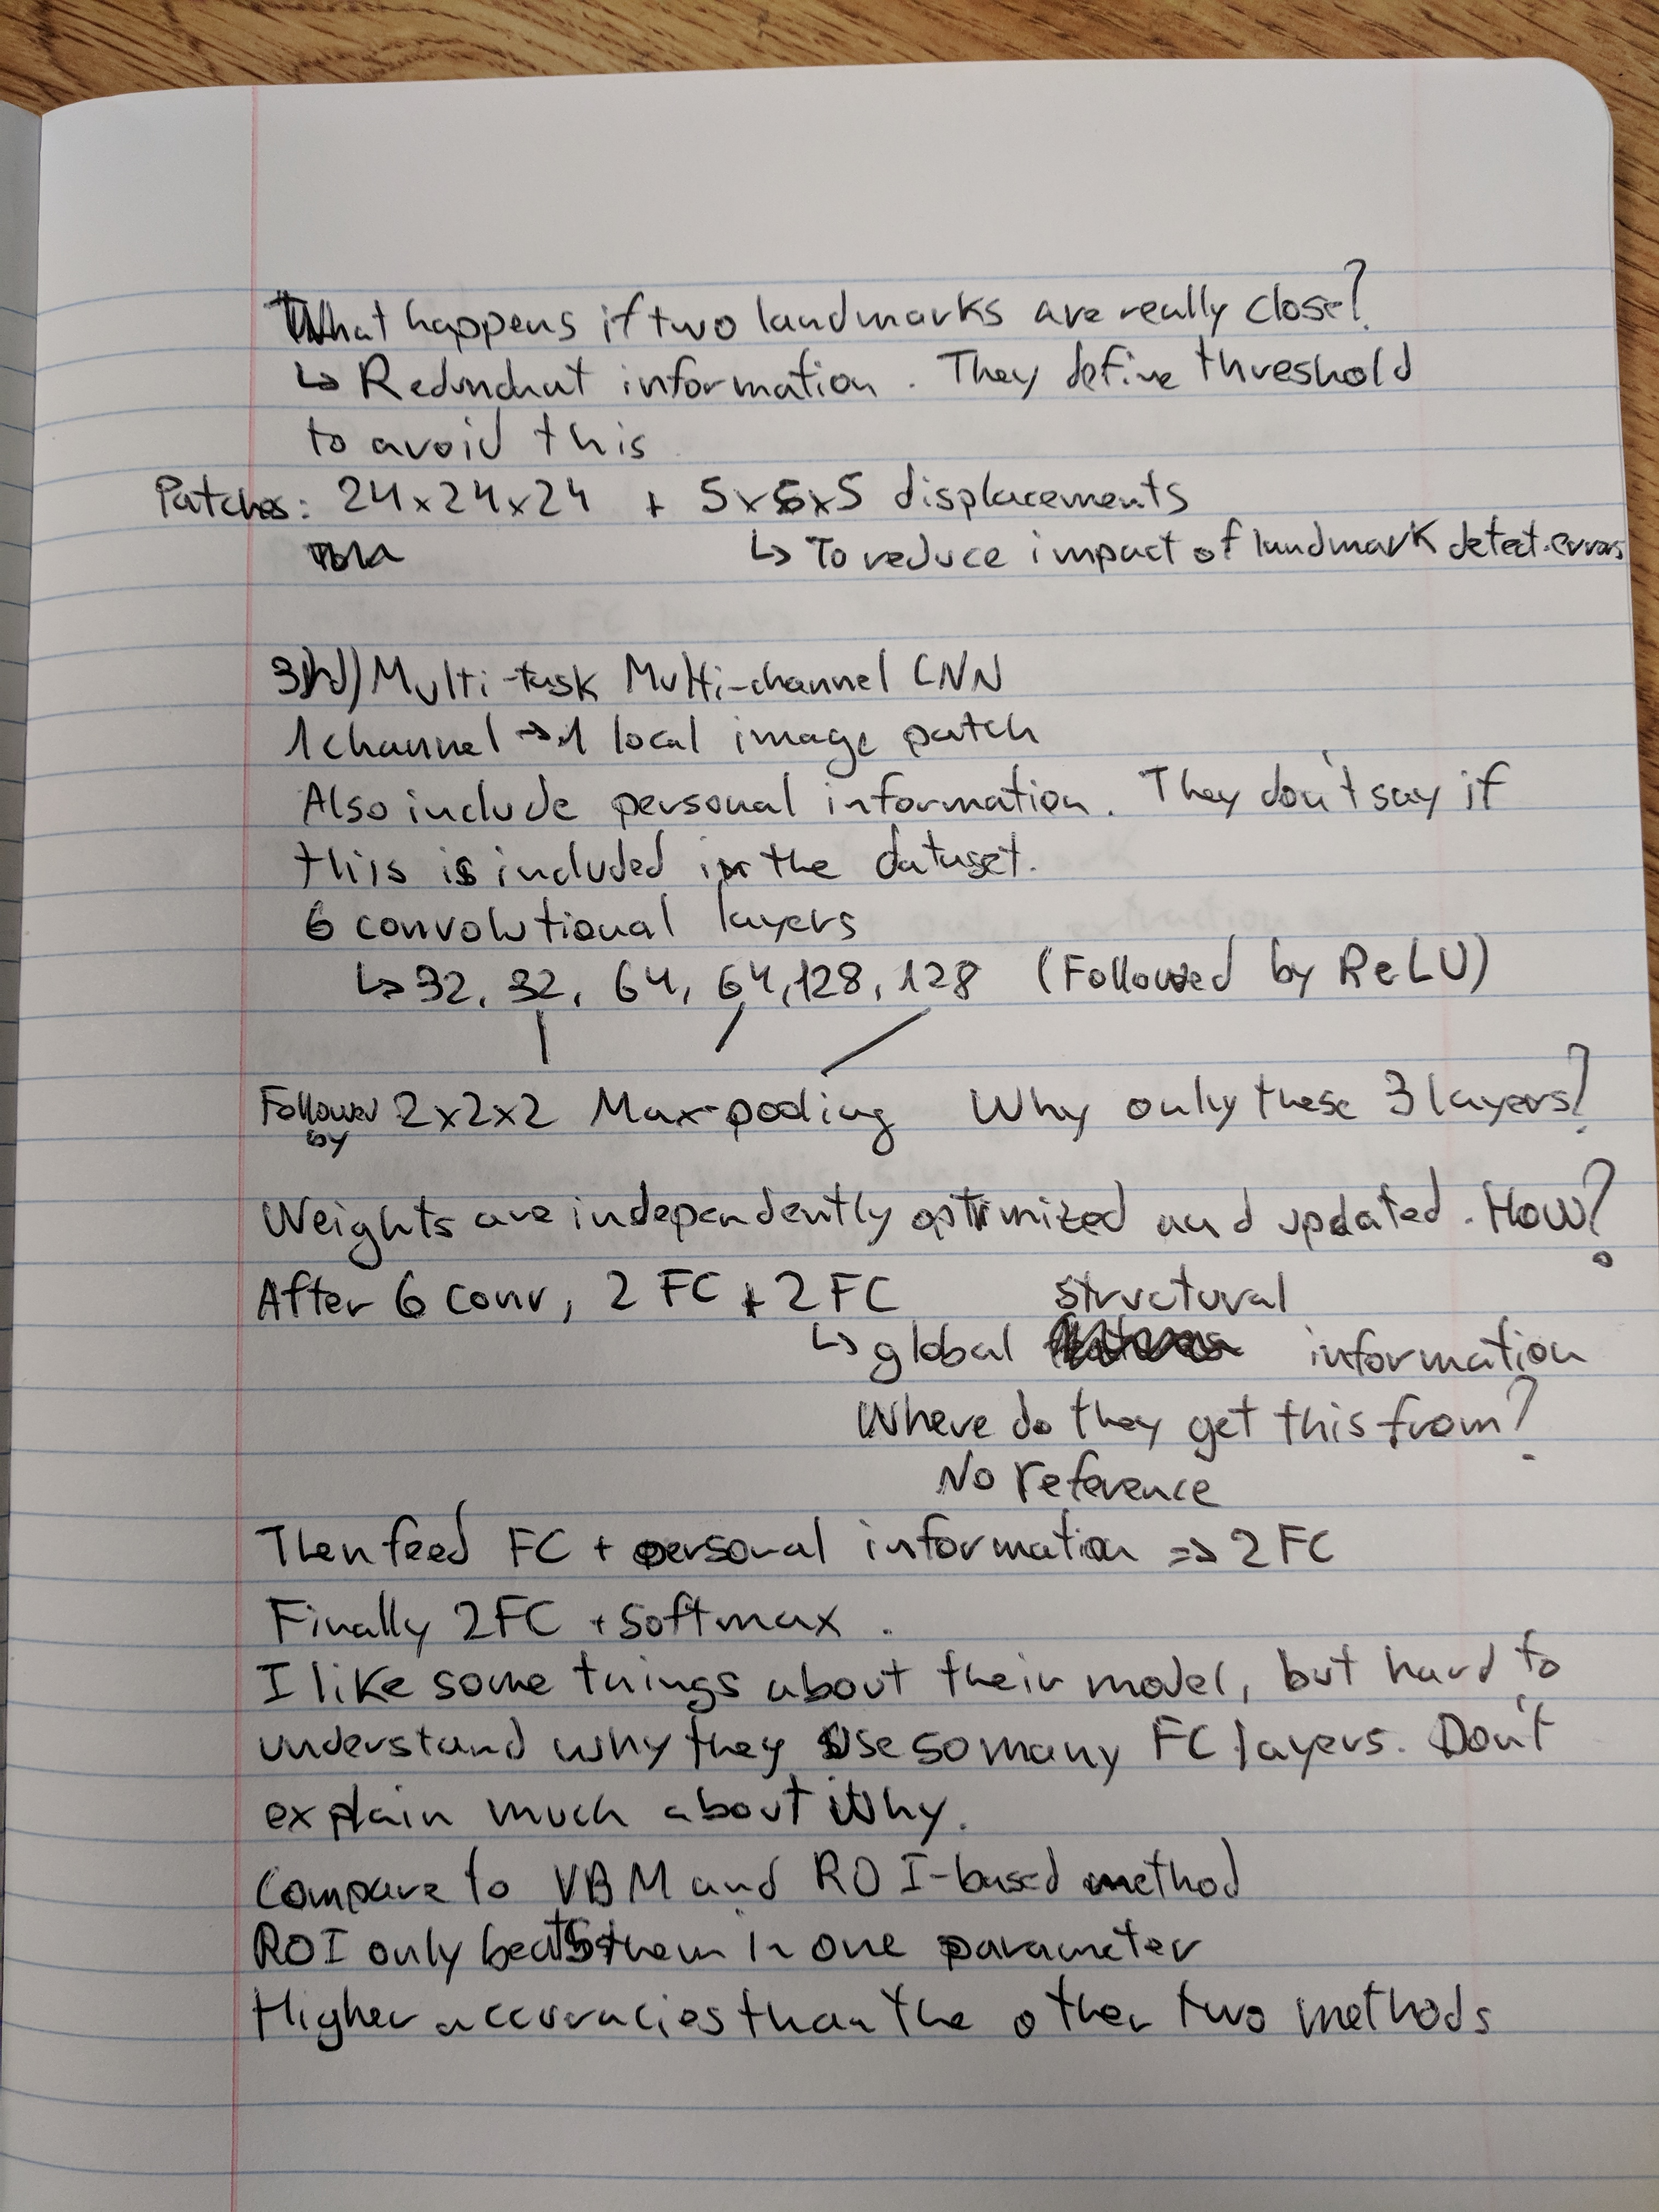
\includegraphics[width=10cm]{paper1_2.jpg}
\caption{Picture 2 for first paper}
\label{fig:paper1_2}
\end{figure}

\begin{figure}[h]
\centering
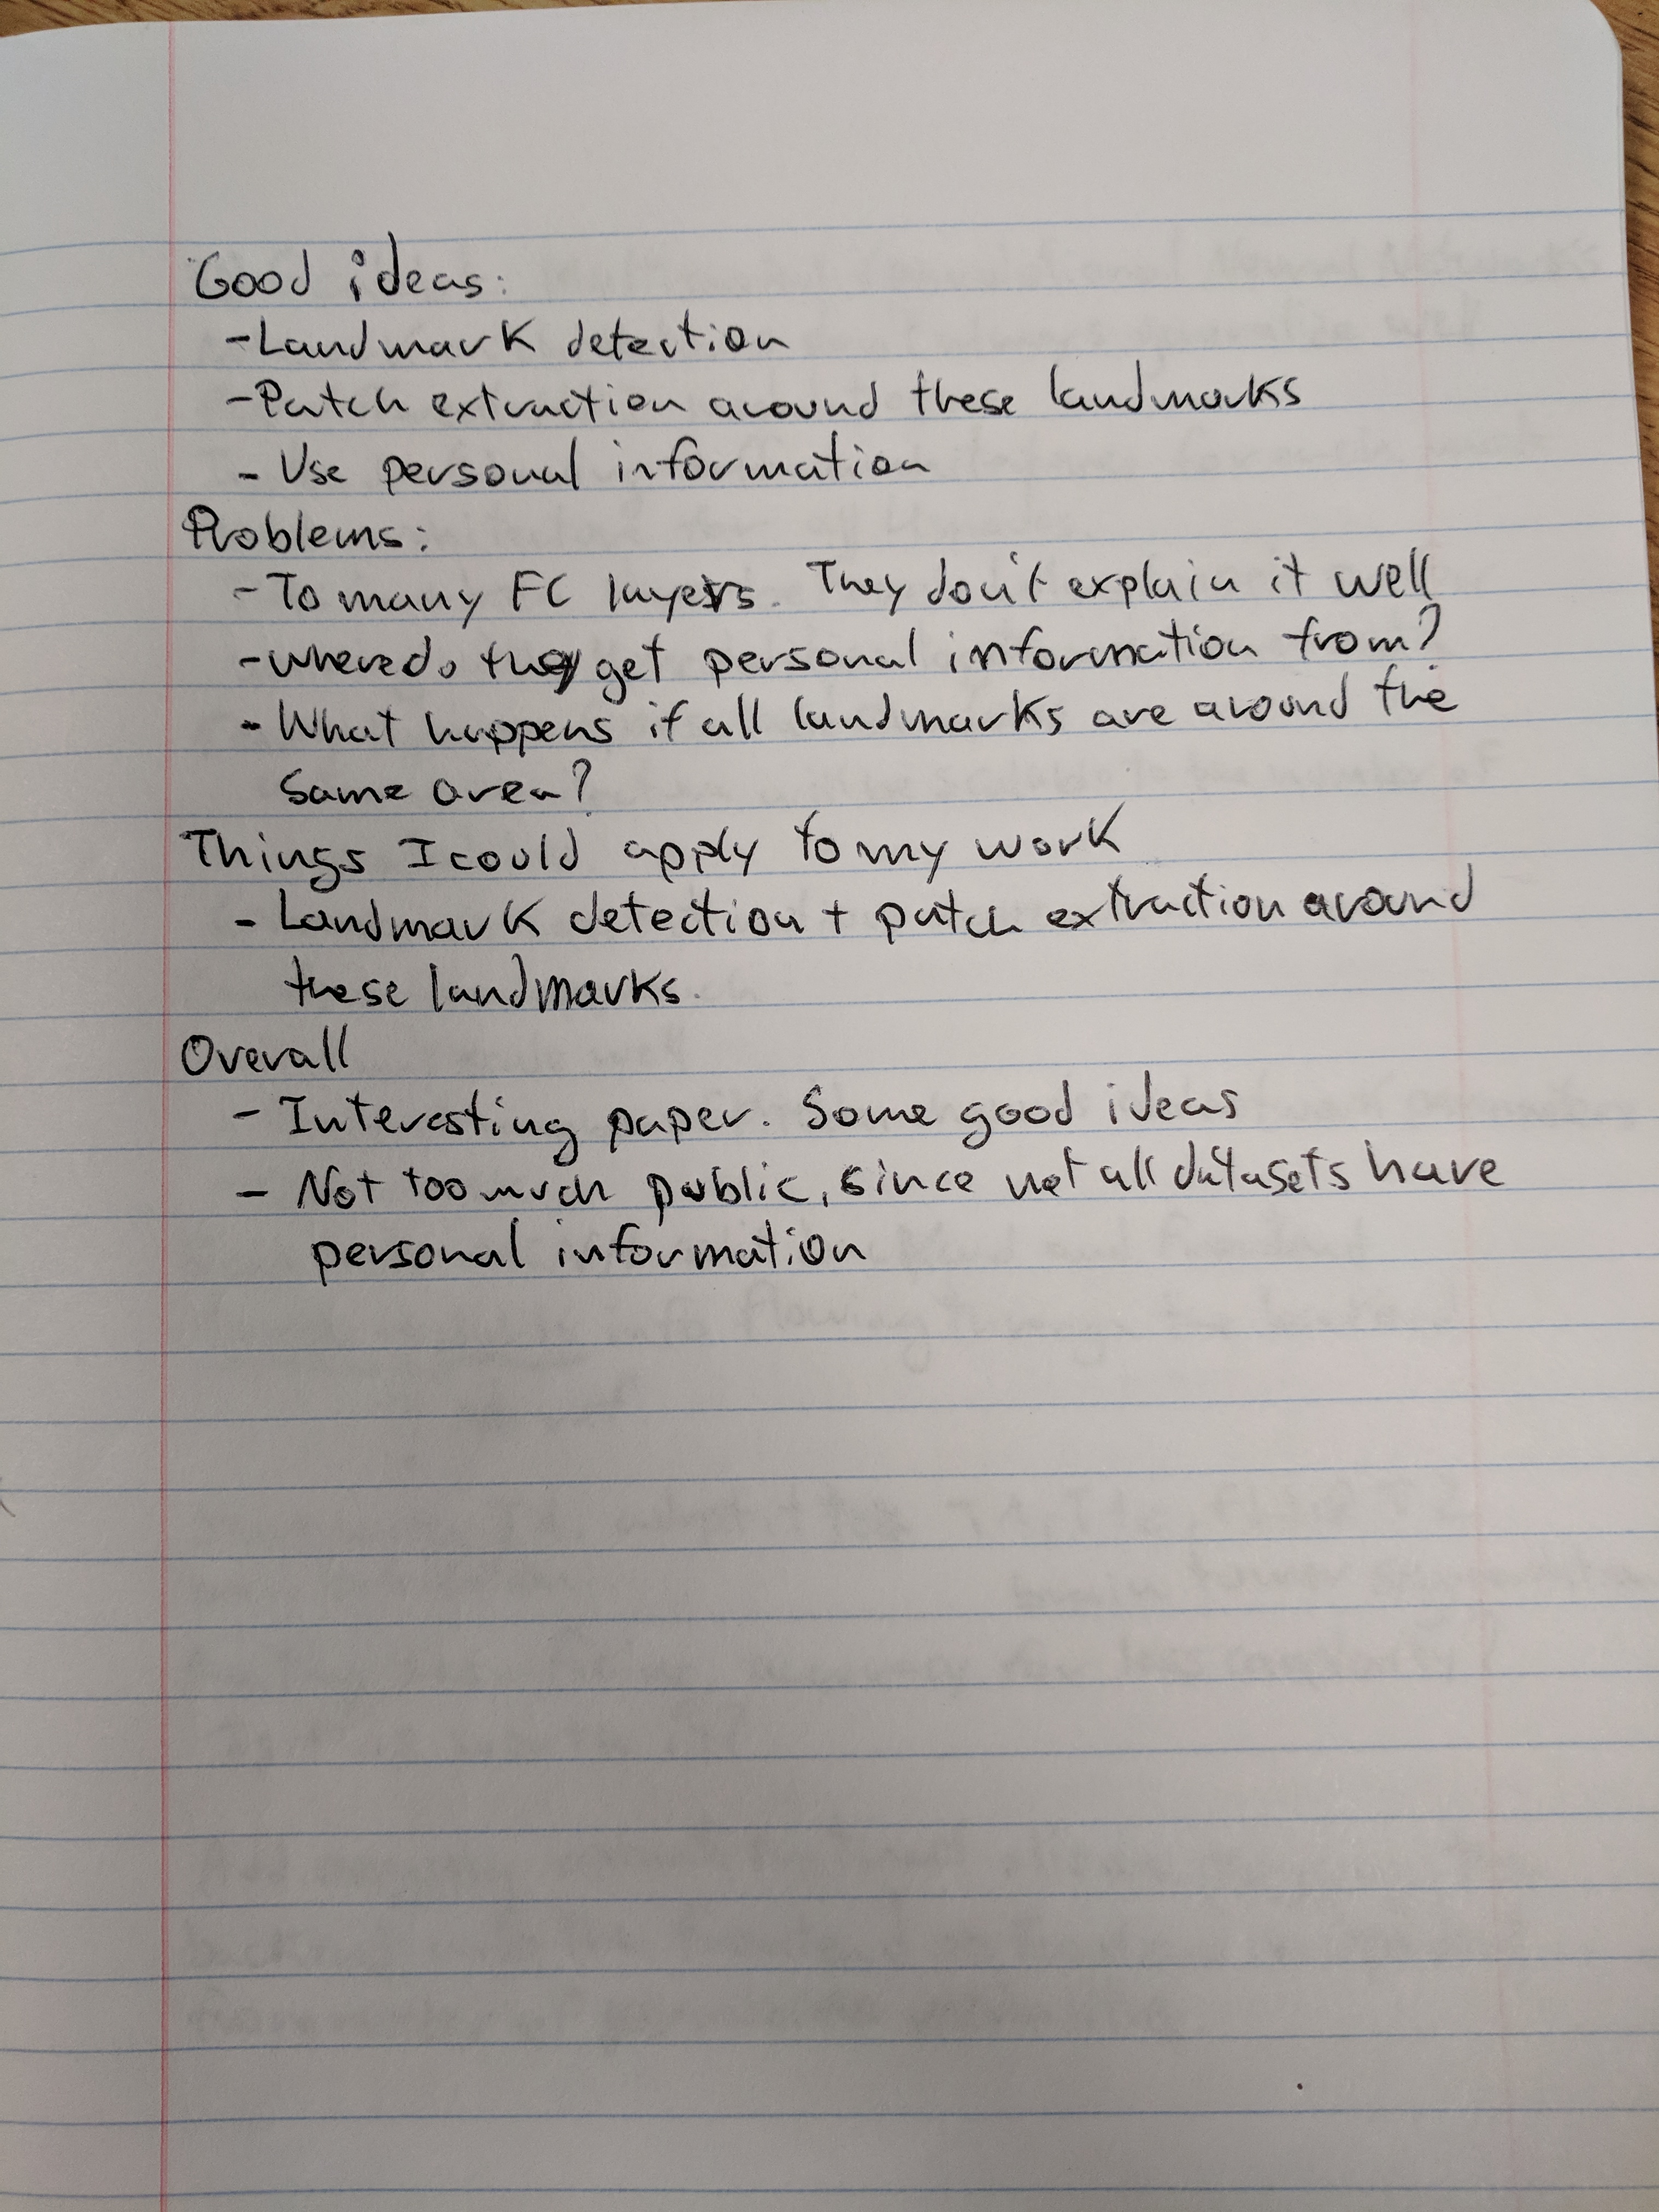
\includegraphics[width=10cm]{paper1_3.jpg}
\caption{Picture 3 for first paper}
\label{fig:paper1_3}
\end{figure}

The second paper that I have decided to critically and creatively read is the one from L. Fidon et al. \cite{10.1007/978-3-319-66179-7_33}. I have made handwritten notes, so I'll include them in figures.

\begin{figure}[h]
\centering
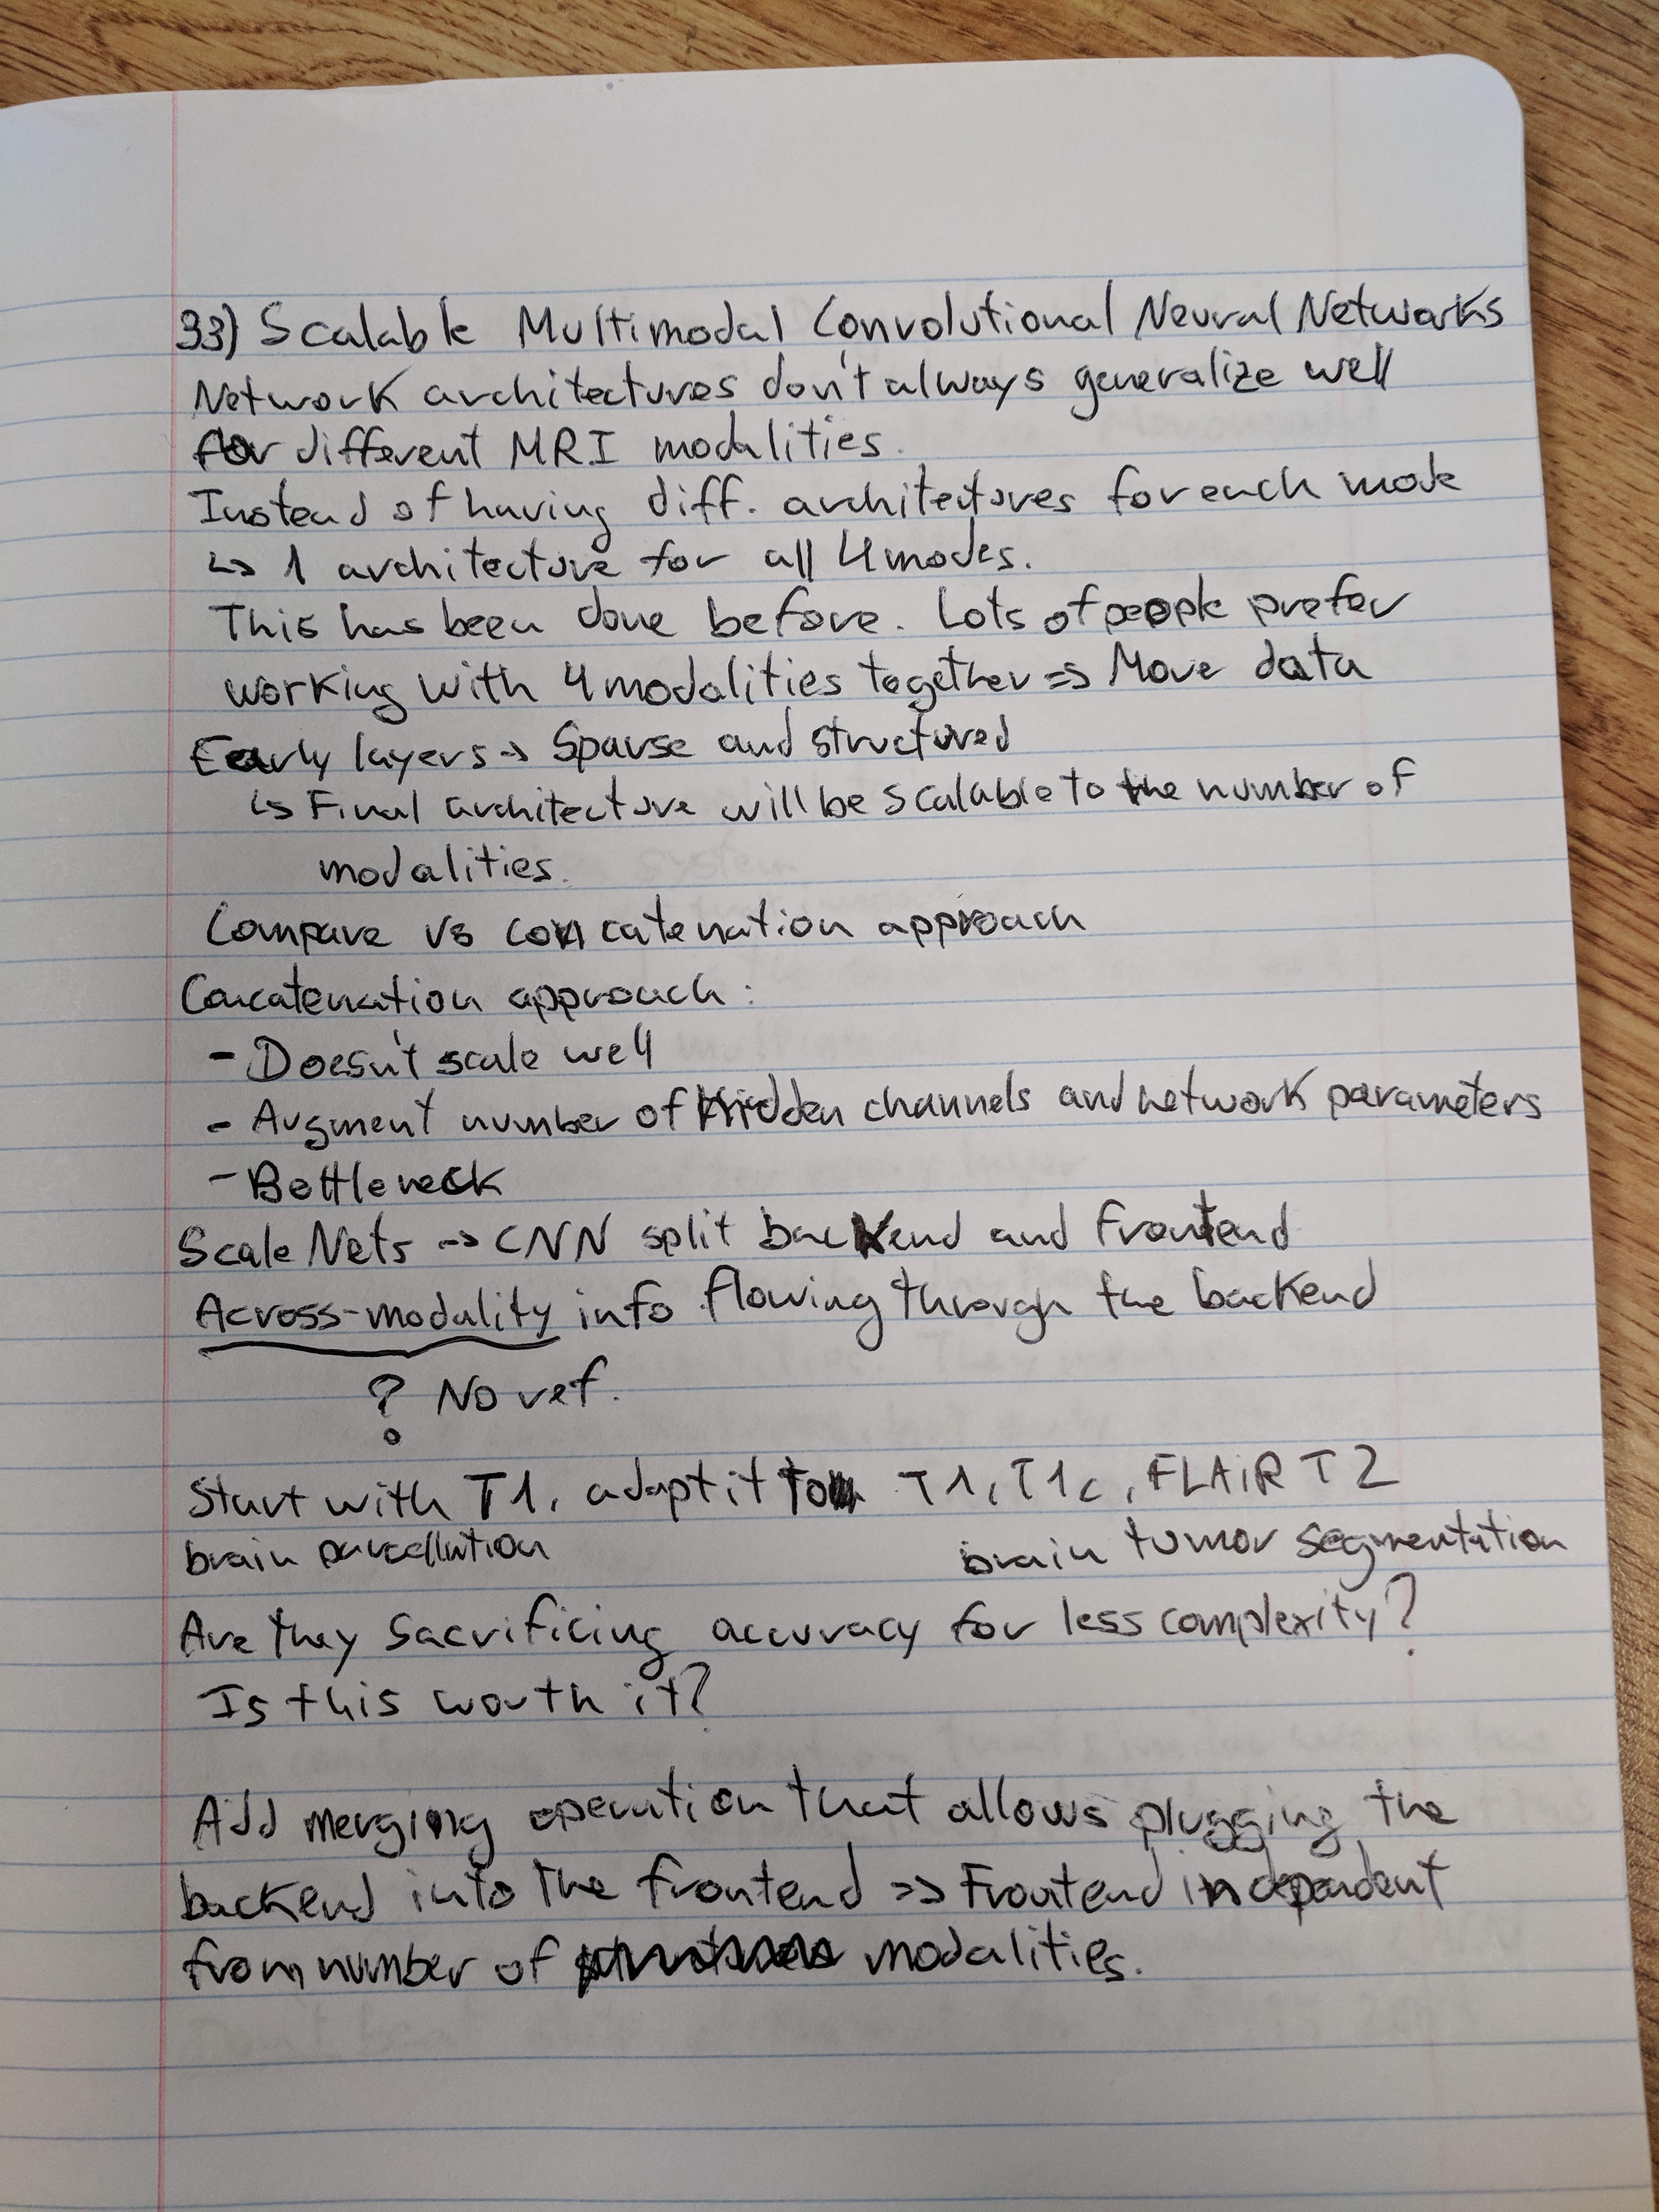
\includegraphics[width=10cm]{paper2_1.jpg}
\caption{Picture 1 for second paper}
\label{fig:paper2_1}
\end{figure}

\begin{figure}[h]
\centering
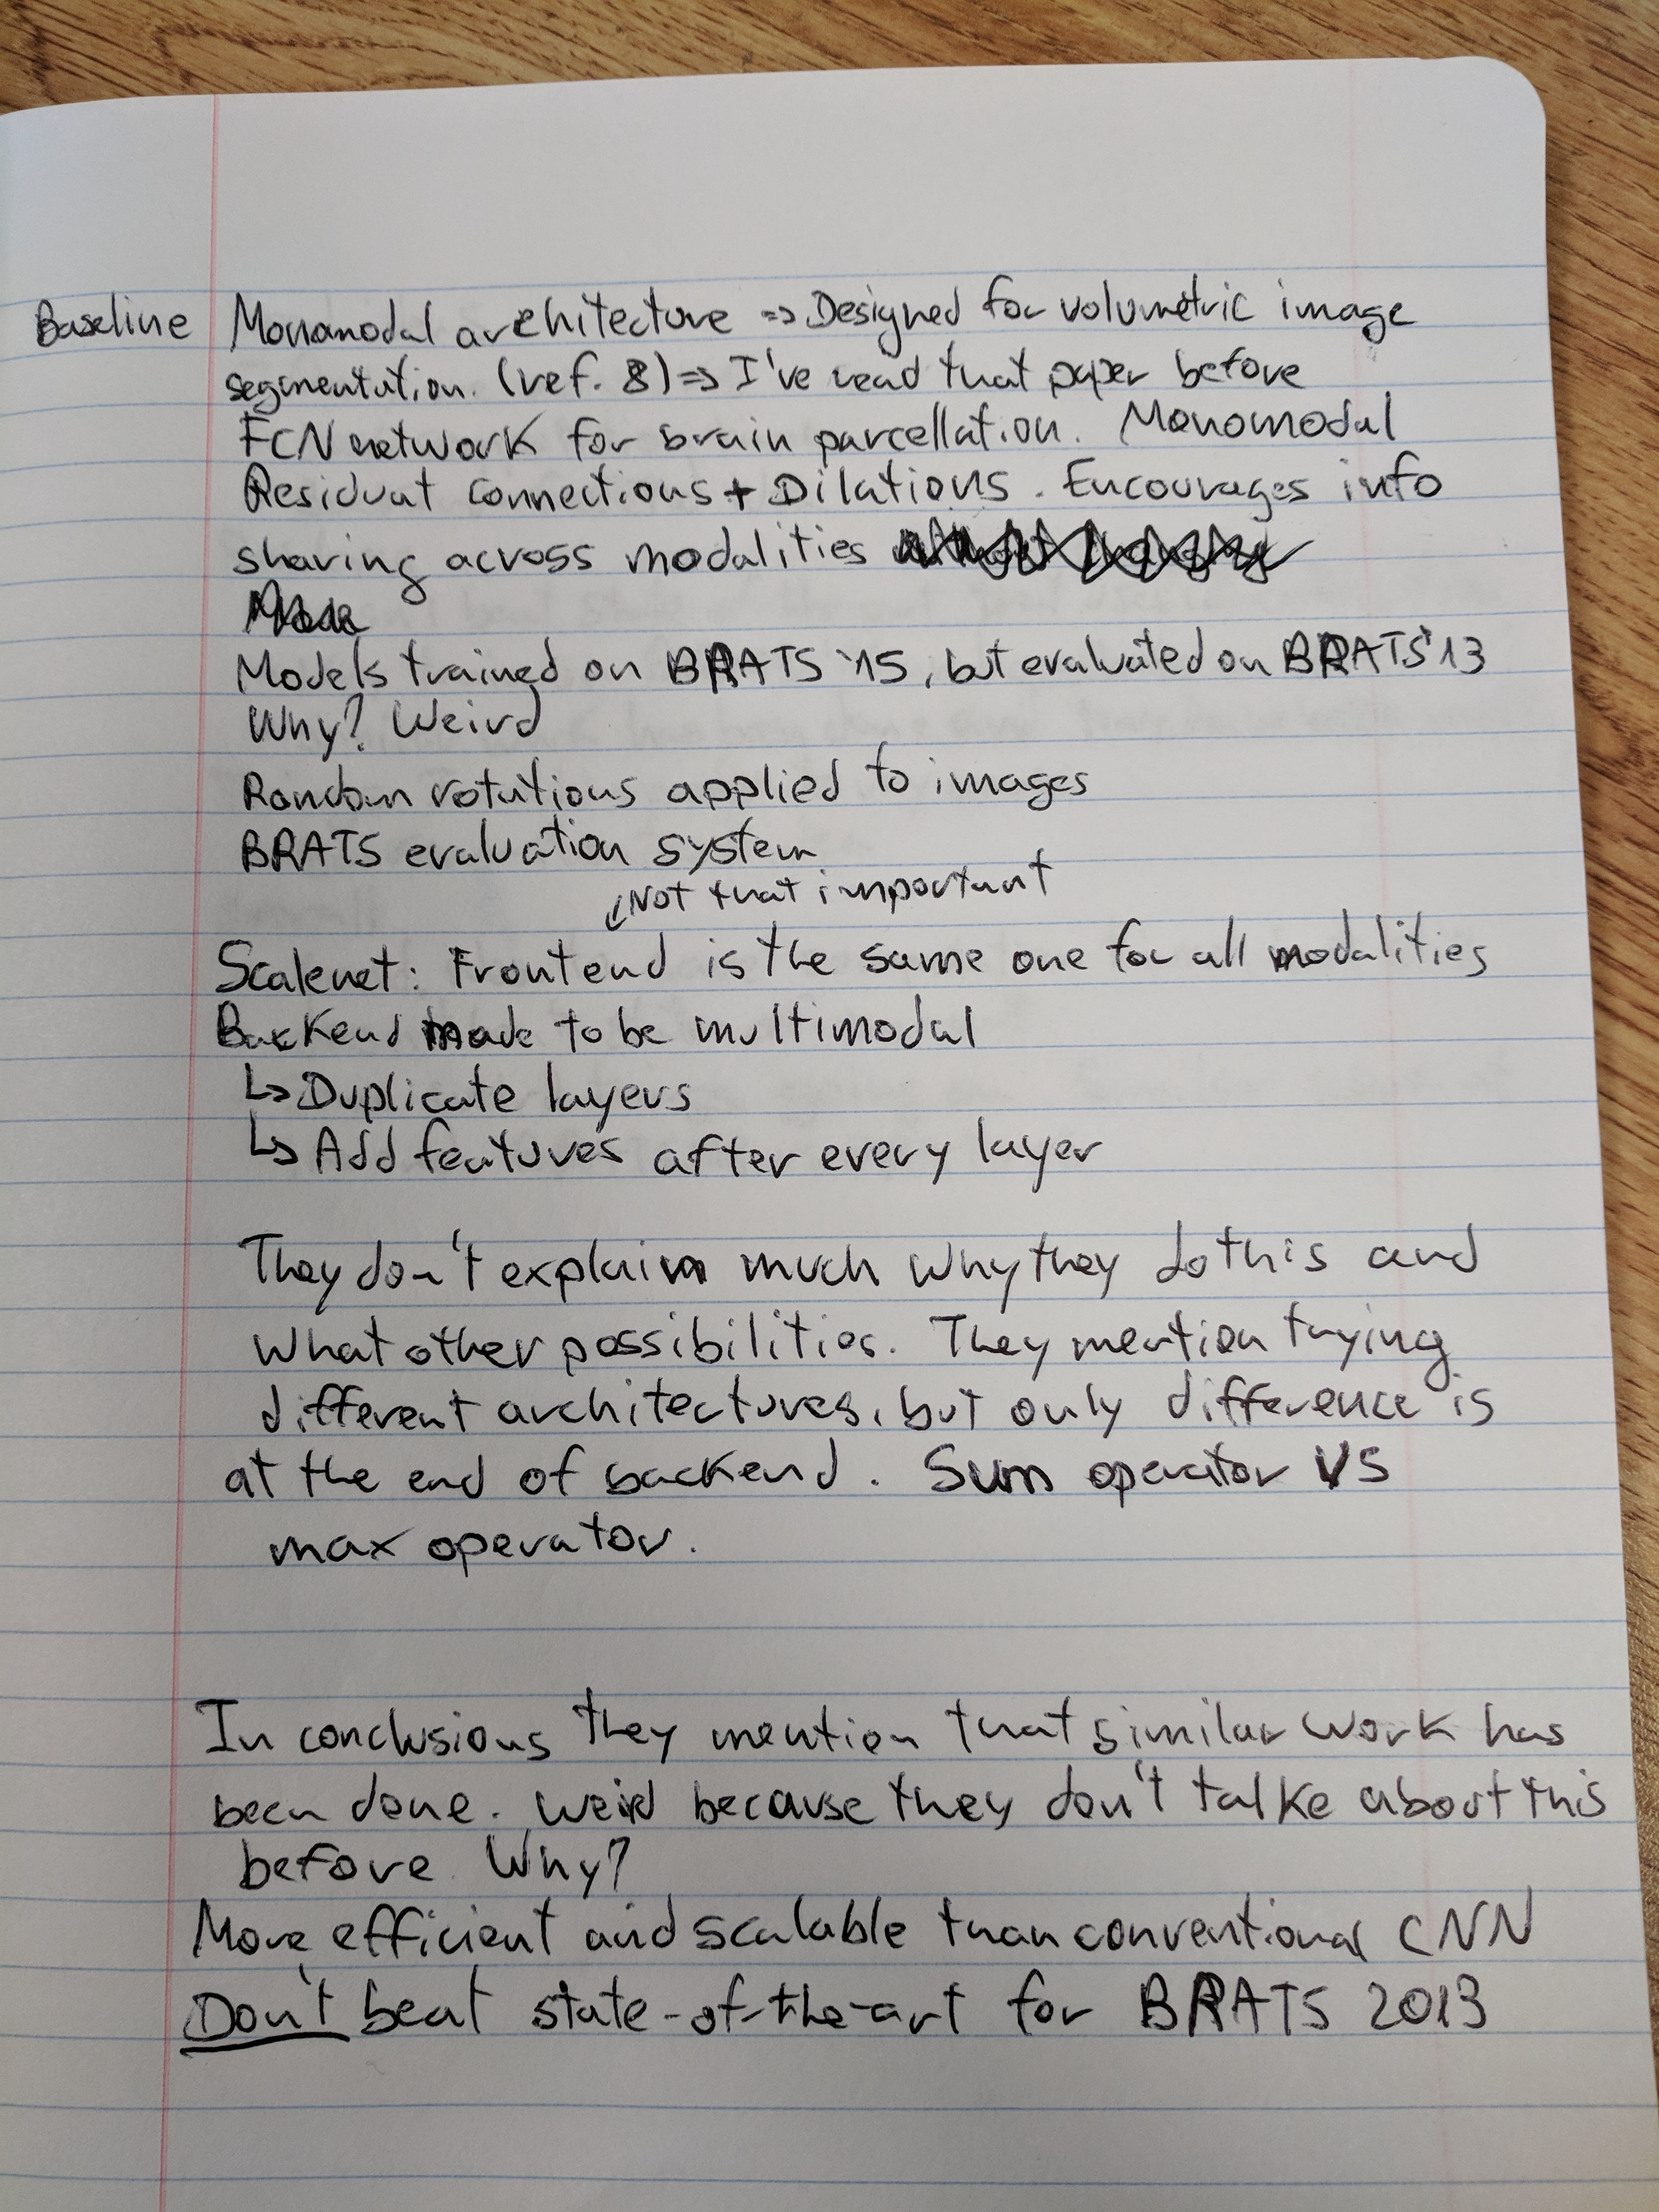
\includegraphics[width=10cm]{paper2_2.jpg}
\caption{Picture 2 for second paper}
\label{fig:paper2_2}
\end{figure}

\begin{figure}[h]
\centering
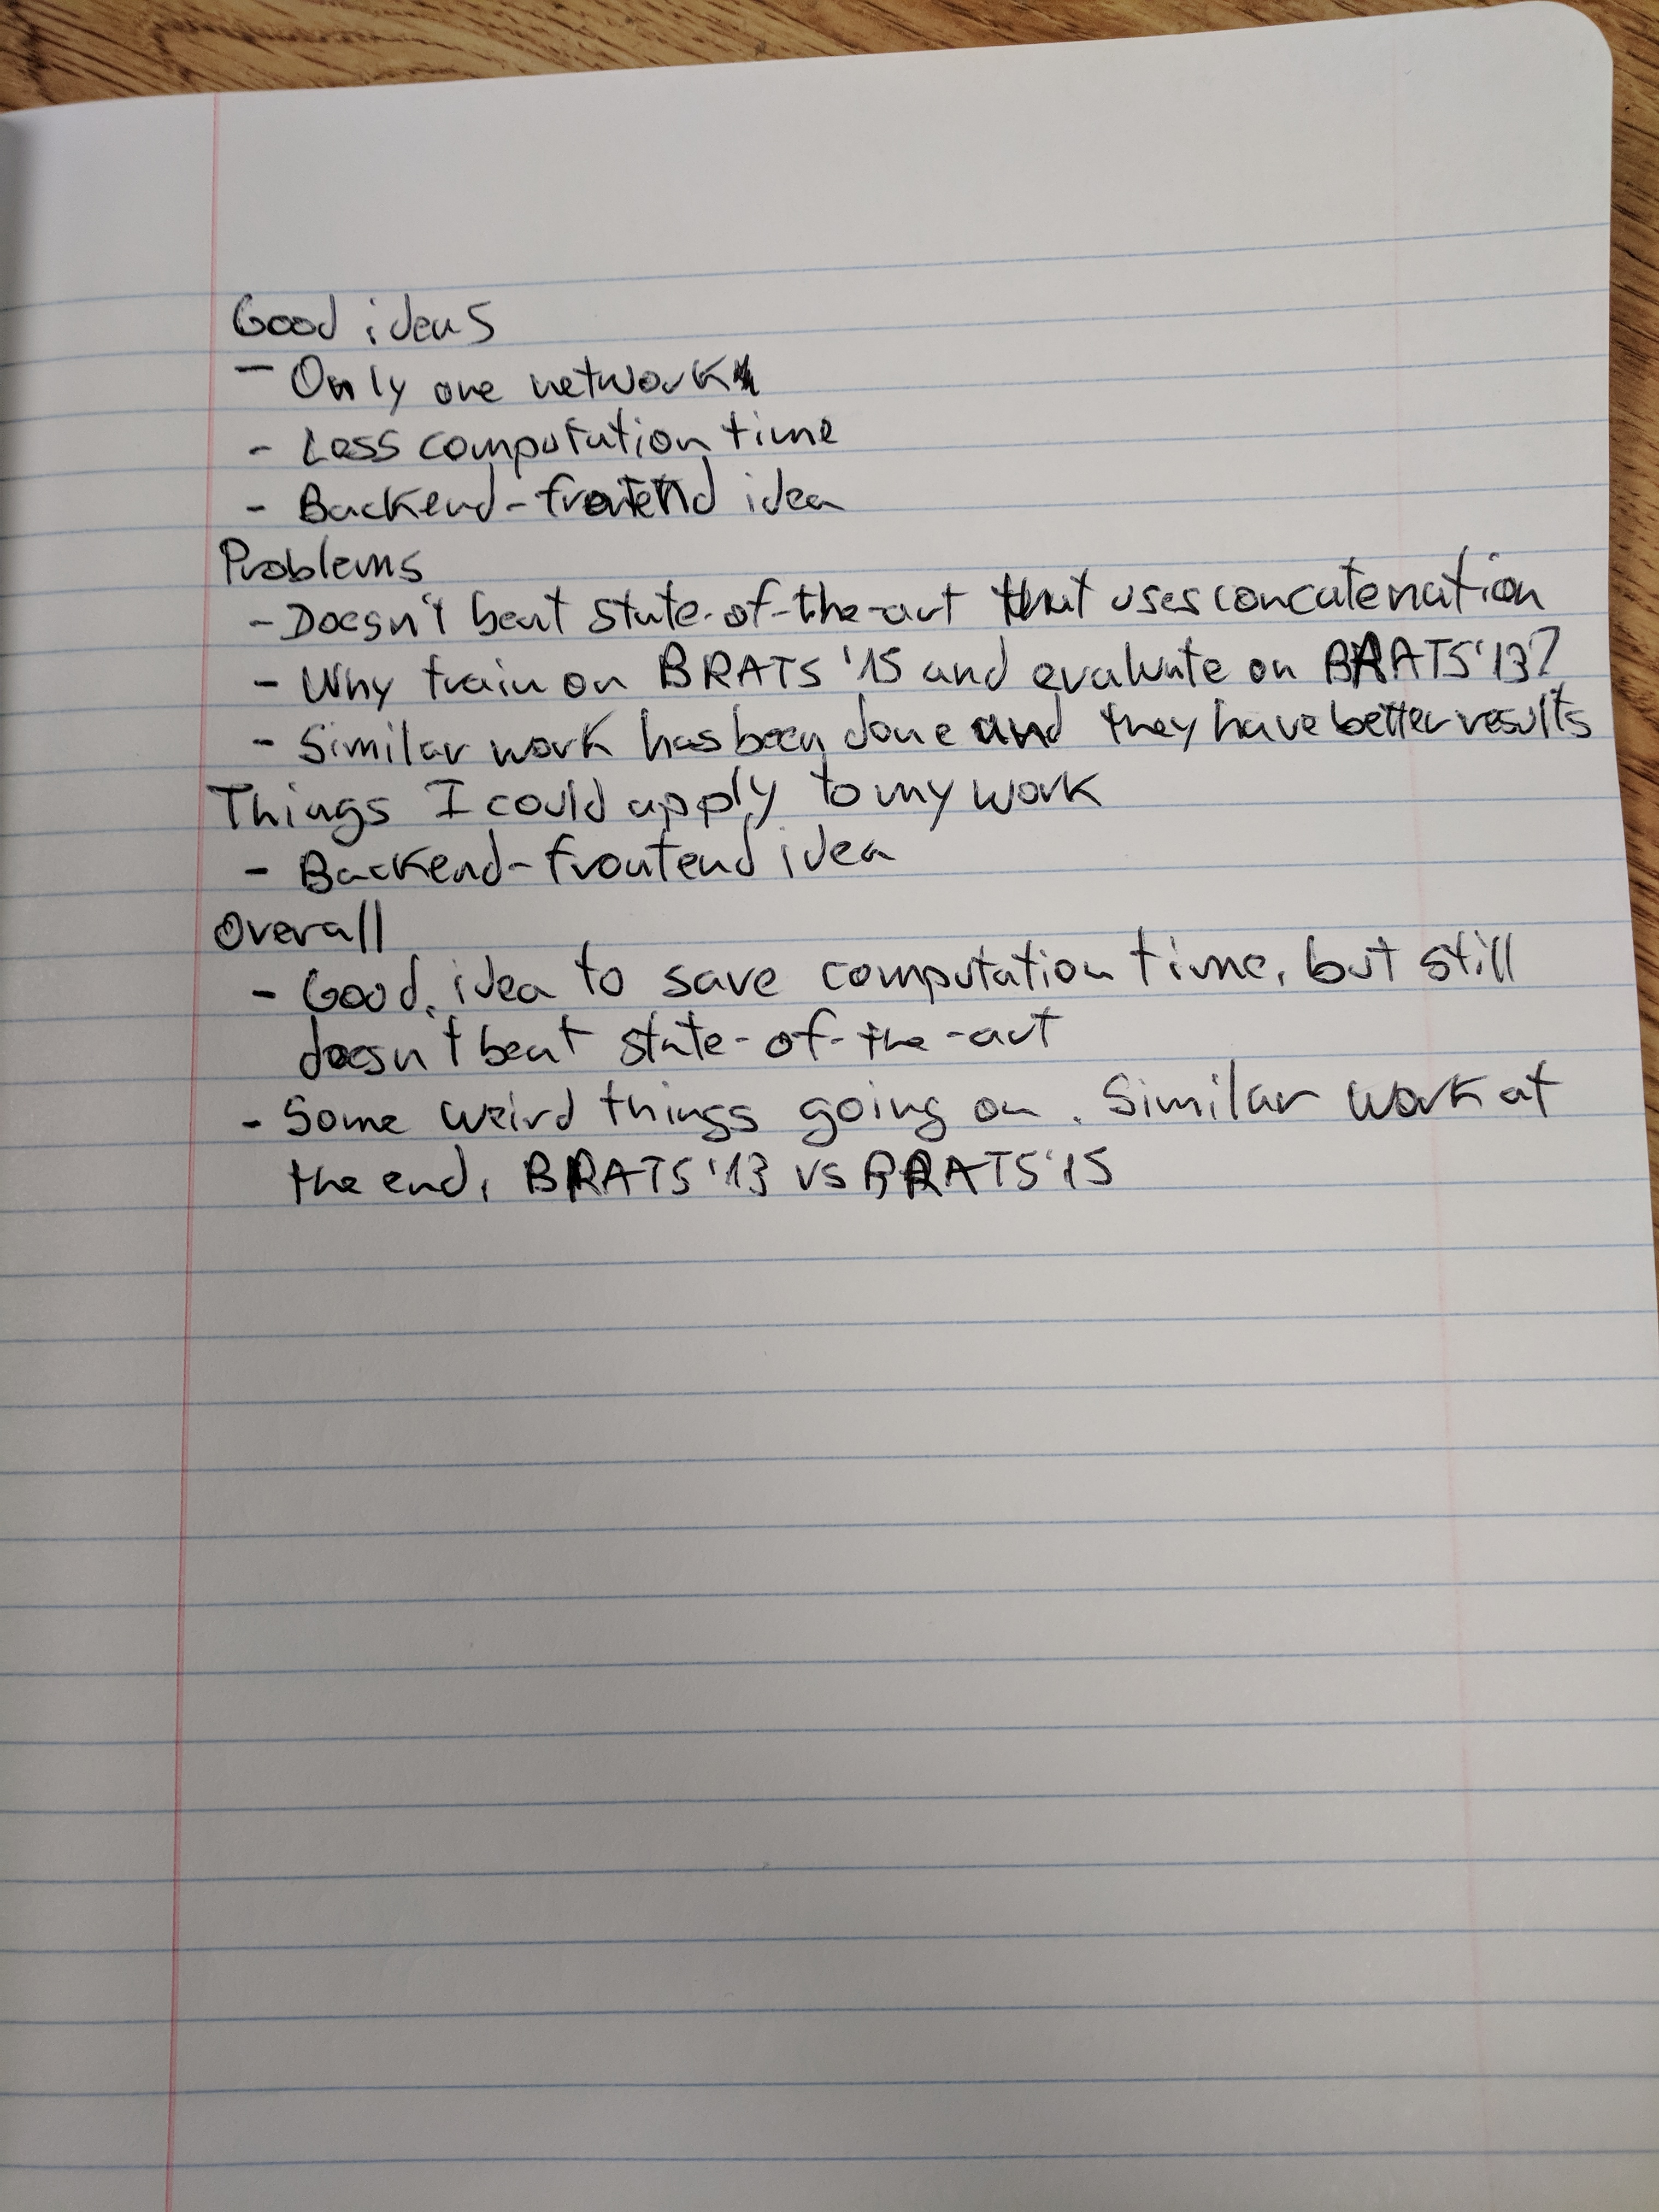
\includegraphics[width=10cm]{paper2_3.jpg}
\caption{Picture 3 for second paper}
\label{fig:paper2_3}
\end{figure}

%The last section is references.. which should start with the citation for the primary conference, plus the citations for have all the papers from the browse, with the timing notes.

%DONE

All the papers have been extracted from \cite{MICCAI}, which is the 3rd part of the Proceedings from MICCAI 2017. 
Papers that I have decided to scan \cite{10.1007/978-3-319-66179-7_1,10.1007/978-3-319-66179-7_5,10.1007/978-3-319-66179-7_10,10.1007/978-3-319-66179-7_26,10.1007/978-3-319-66179-7_27,10.1007/978-3-319-66179-7_33,10.1007/978-3-319-66179-7_36,10.1007/978-3-319-66179-7_38}

%All of this should be in your git repo as a directory, upload the pdf here. 

\nocite{*}

\printbibliography

\end{document}

